\emph{For the following experiments, $\lambda=11$.}\\
\\
Fig. \ref{fig:umulevolution} below shows the evolution of the value of $J^{*}$ with $U_{mul}$.
\begin{figure}[!h]
	\centering
	\caption{Evolution of $J^{*}$ with $U^{mul}$}
	\label{fig:umulevolution}
	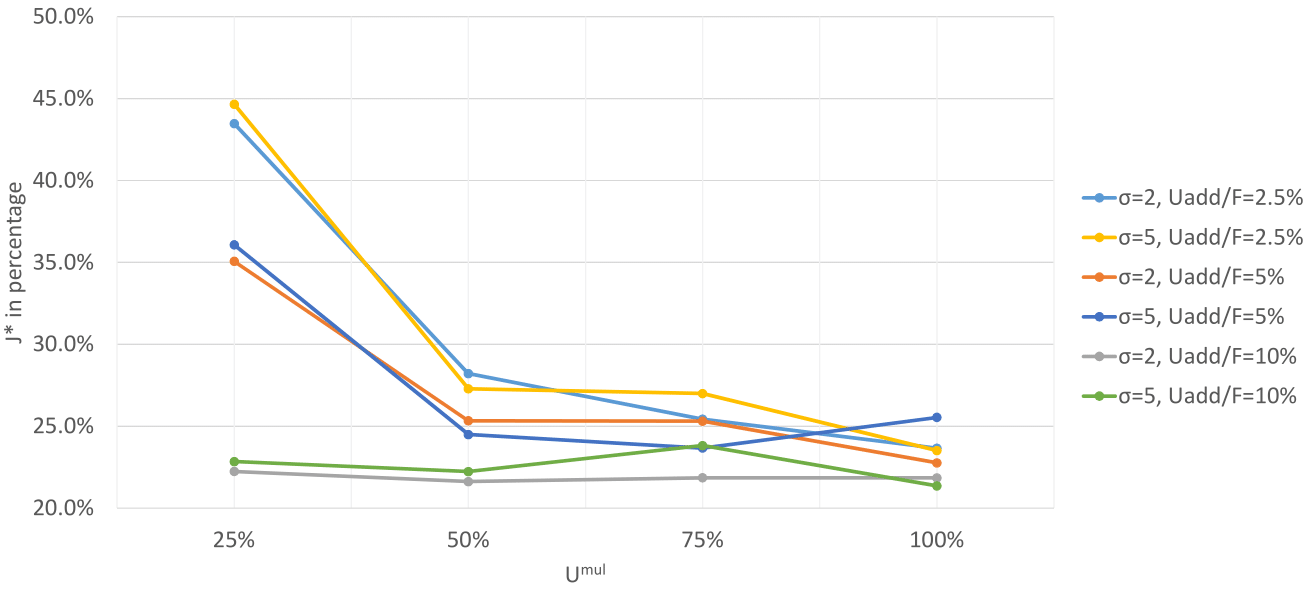
\includegraphics[width=7in]{figures/umul.png}
\end{figure}\\
As intuitively guessed, the more uncertainty i.e. freedom to the knobs there is, the smaller $J^{*}$ is.\\
More precisely, the tendencies observed are the following :
\begin{itemize}
	\item If $U^{add}$ is not too big (i.e. doesn't override the effect of $U^{mul}$), there is a minimum threshold on $U^{mul}$ for $J^{*}$ to be reasonably small : in our case, $U^{mul}$ around $25\% $ doesn't give satisfactory $J^{*}$ values ($35\% $ and $45\% $). It enters in an acceptable range if $U^{mul}\geq 50\% $. This shows the importance of the uncertainty, due to the lack of precision of the whole : a multiplicative uncertainty of $25\% $ or less is not enough.
	\item There is no real difference for the effect of $U^{mul}$ between $50\% $ and $75\% $: they are the typical executions.
	\item When the multiplicative uncertainty is very big, i.e. $U^{mul}=100\% $ (minimums are zero i.e. the physical minimums; and the maximums correspond to twice the partially monitored segments flow demands), the result seem to slightly improve. However, one run ($\sigma=5$ and $\frac{U^{add}}{\widetilde{F}}=5\% $) shows that it is not always the case :  the feasible space becomes very big and CMA-ES is not guided at all. In fact, as we will observe on the congestion pattern contour plots in this case, the results are not satisfactory.
\end{itemize} 
Below are 4 groups of figures. They display especially, for each of the 4 values of $U^{mul}$, how the resulting congestion pattern fitting and the history of the knobs trough the execution evolve with $U^{add}$ and $\sigma$.\\
\begin{figure}[!h]
	\centering
		\caption{$\mathbf{U_{mul}=25\%}$. Congestion pattern matching plots : evolution with $U_{add}$ and $\sigma$.}
	\label{fig:umulcp25}
	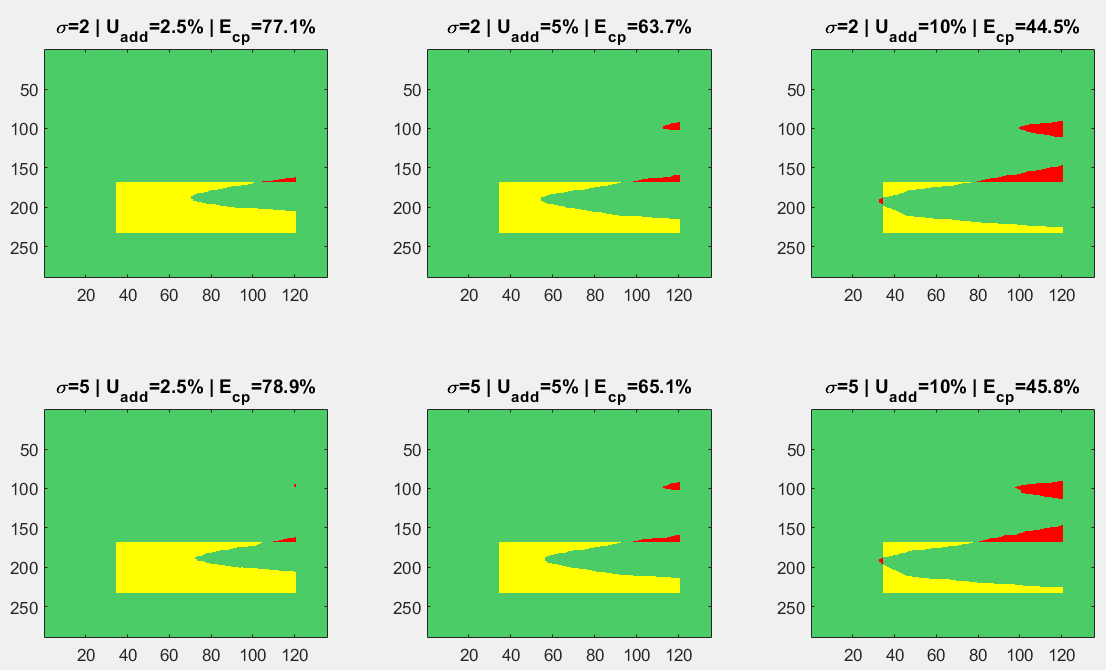
\includegraphics[width=7in]{figures/results_figures/Umul/cp_Umul_25_lambda_11.png}
\end{figure}	
\begin{figure}[!h]
	\centering
	\caption{$\mathbf{U_{mul}=25\%}$. Knobs history plots : evolution with $U_{add}$ and $\sigma$.}
	\label{fig:umulknobs25}
	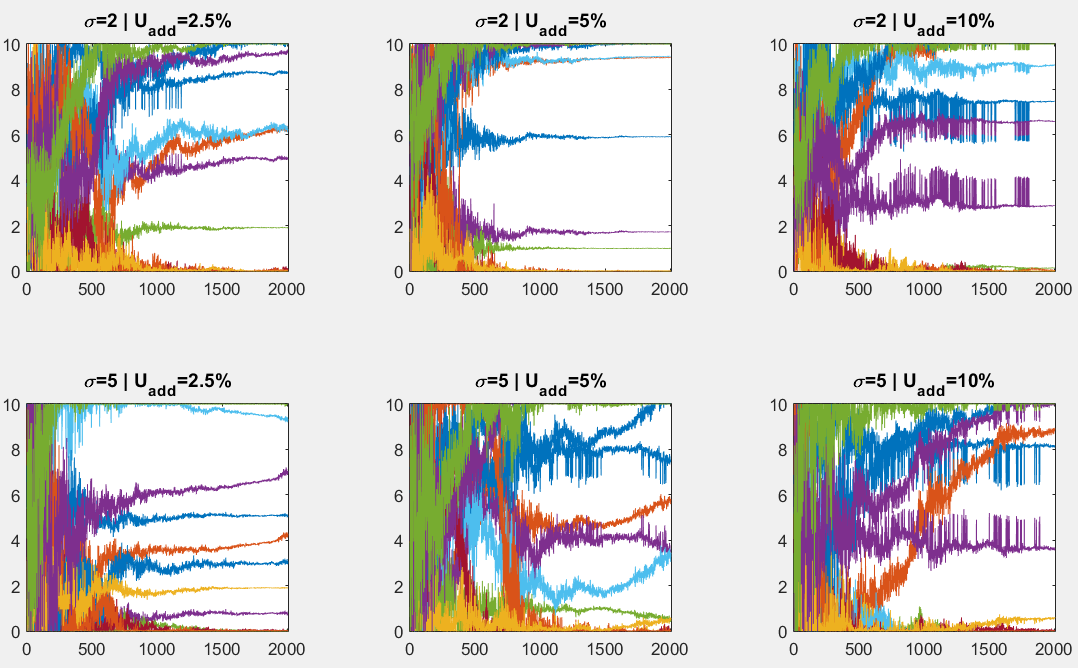
\includegraphics[width=7in]{figures/results_figures/Umul/knobs_Umul_25_lambda_11.png}
\end{figure}
\begin{figure}[!h]
	\centering
	\caption{$\mathbf{U_{mul}=25\%}$. $E_{VHT}$ evolution plot with $U^{add}=2.5\% $.}
	\label{fig:badvht}
	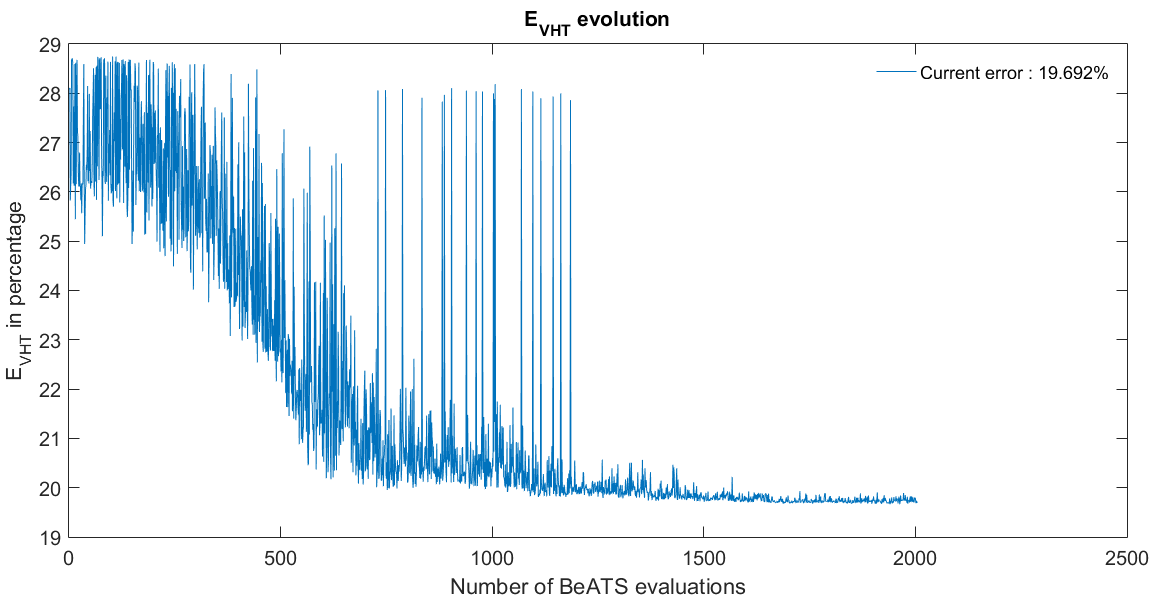
\includegraphics[width=7in]{figures/results_figures/Umul/bad_vht.png}
\end{figure}		
\newpage
\emph{$U^{mul}=25\% $}: Fig. \ref{fig:umulcp25}, with $U^{mul}=25\% $, shows the effect on the result of excessively tight constraints.  With $U^{add}=2.5\% $ and $5\% $ (two first columns), $\mathscr{C}$ cannot grow enough to fill $\widetilde{\mathscr{C}}$, which is responsible for a very high $E_{CP}^{*}$.\\
In addition, Fig. \ref{fig:badvht} shows that, with these parameters, $E_{VHT}$ converges to an unacceptable $20\% $ (it converges below $5 \% $ in all other configurations).
In the last column, $U^{add}=10\% $ gives a good space to all the knobs (many of them having their physical boundaries $\mathscr{B}$). In this case, $U^{mul}=25\% $ has no effect, which is the reason for the good "typical" result obtained.\\
To summarize, as highlighted previously by Fig. \ref{fig:umulevolution}, setting $U^{mul}$ to a value smaller than a significant threshold ($25\% $ is quite high !) expels the good acceptable solutions from the feasible space.\\

There is nothing clear to conclude from the knobs evolution on Fig. \ref{fig:umulknobs25}., except that many end up on their boundaries (up to 8 of 12 !), which reflects that they were set too tight i.e. that we describe a far-from-reality situation.
\newpage
\begin{figure}[!h]
	\caption{$\mathbf{U_{mul}=50\%}$. Congestion pattern matching plots : evolution with $U_{add}$ and $\sigma$.}
	\label{fig:umulcp50}
	\centering
	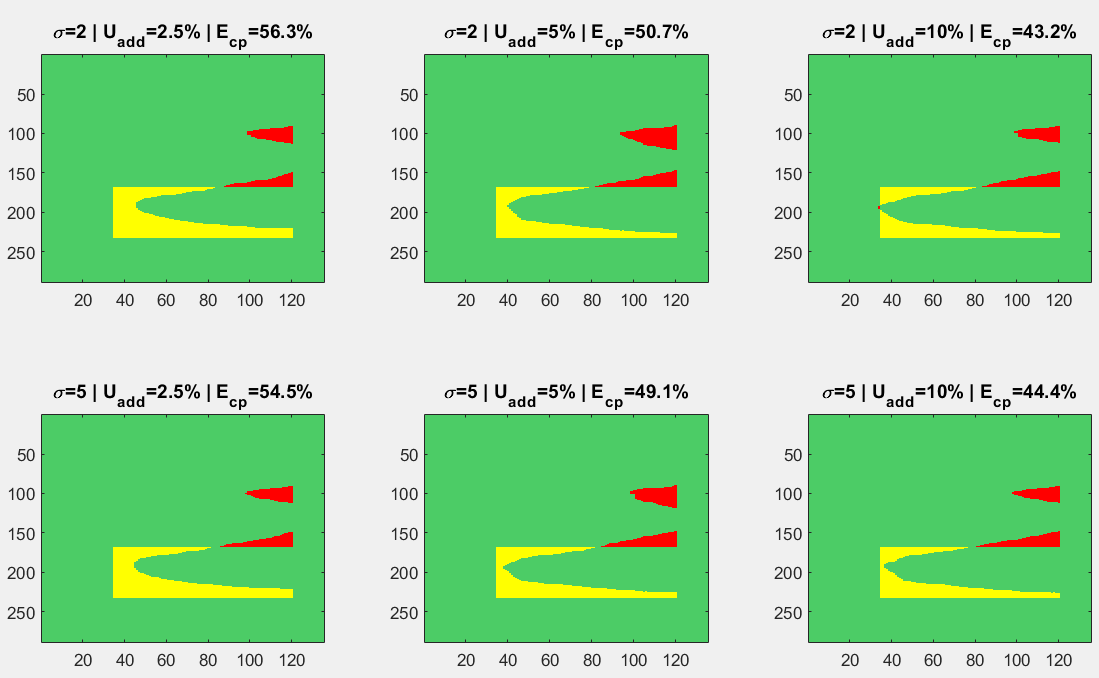
\includegraphics[width=6.8in]{figures/results_figures/Umul/cp_Umul_50_lambda_11.png}
\end{figure}
\begin{figure}[!h]
	\caption{$\mathbf{U_{mul}=50\%}$. [0-10] knobs history plots : evolution with $U_{add}$ and $\sigma$.}
	\label{fig:umulknobs50}
	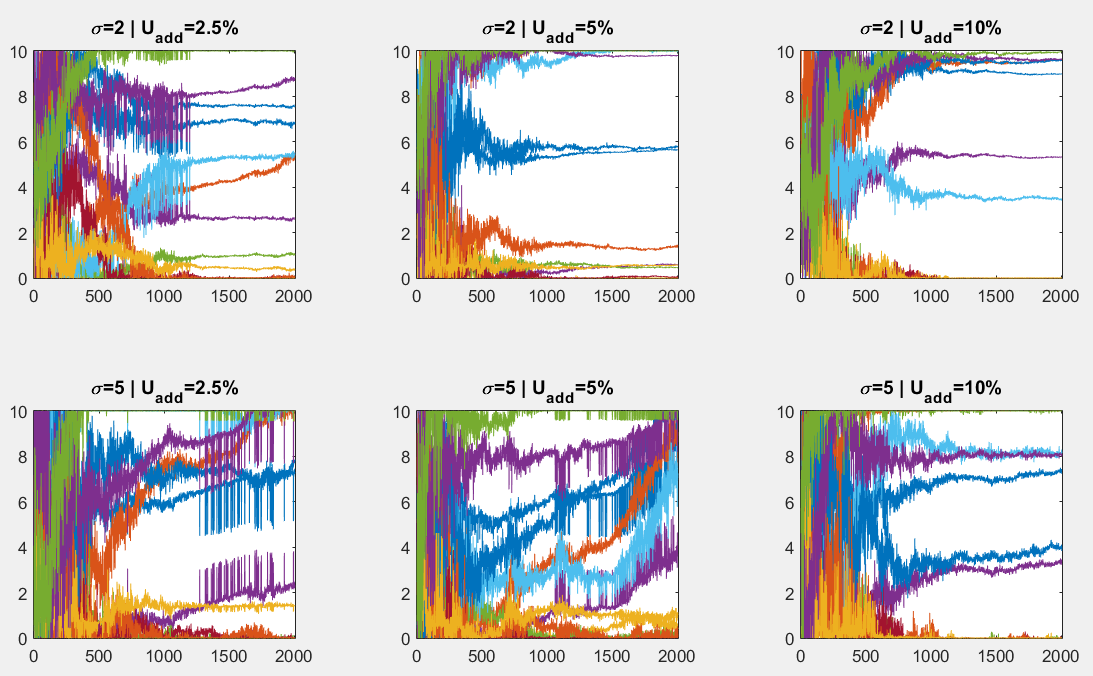
\includegraphics[width=7in]{figures/results_figures/Umul/knobs_Umul_50_lambda_11.png}
\end{figure}	
\emph{$U^{mul}=50\% $}: We observe in Fig. \ref{fig:umulcp50} only typical results, with, as expected, a slight improvement while loosing the $U^{add}$ constraint.\\
In Fig. \ref{fig:umulknobs50}, there are more situations than previously with many knobs converging to another value than their  boundaries. We see a situation (middle-down figure) where the knobs did not finish converging, although the result is good : this illustrates the "equivalent global minima" mentioned in \ref{subsec:results_intro}. Some knobs whose action do not affect $\mathscr{C}$ can evolve in a correlated way (e.g. one on-ramp and one off-ramp knob both increase their value), maintaining all the contributions on a constant value. Their variations are therefore invisible to $\mathscr{C}$ and $J$.\\
\newpage
\begin{figure}[!h]
	\centering
	\caption{$\mathbf{U^{mul}=75\%}$. Congestion pattern matching plots : evolution with $U^{add}$ and $\sigma$.}
	\label{fig:umulcp75}
	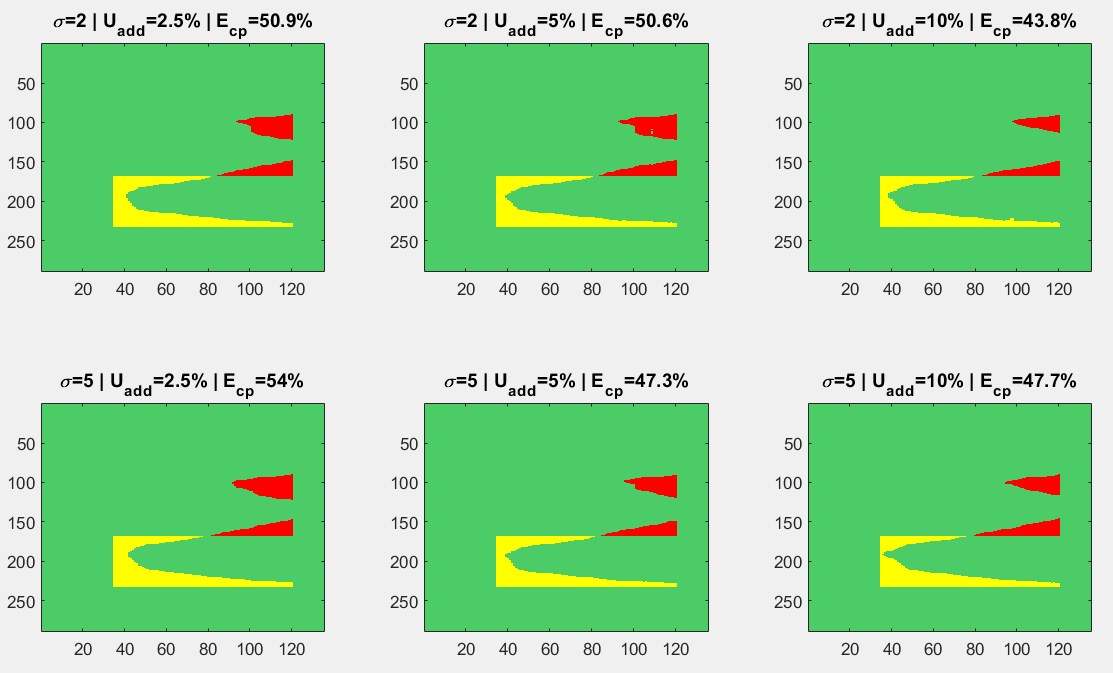
\includegraphics[width=6.8in]{figures/results_figures/Umul/cp_Umul_75_lambda_11.png}
\end{figure}
\begin{figure}[!h]
	\centering
	\caption{$\mathbf{U^{mul}=75\%}$. [0-10] knobs history plots : evolution with $U^{add}$ and $\sigma$.}
	\label{fig:umulknobs75}
	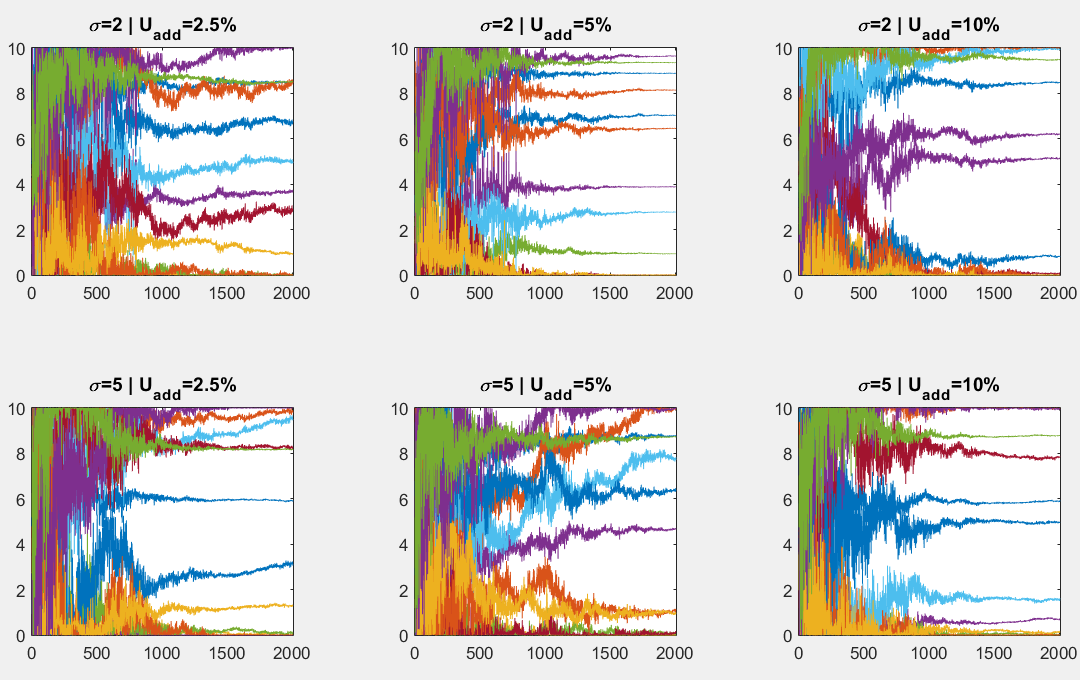
\includegraphics[width=7in]{figures/results_figures/Umul/knobs_Umul_75_lambda_11.png}
\end{figure}	

\emph{$U^{mul}=75\% $}: Fig. \ref{fig:umulcp75} is similar to the preceding Fig. \ref{fig:umulcp50}. Unusual but acceptable congestion shapes that we did not observe before can appear when $U^{add}$ is small and $U^{mul}$  is large. \\
There are many situations in Fig. \ref{fig:umulknobs75}. where many knobs (up to 9 of 12) converge far from their boundaries : this is a desirable situation and is expected, because we loosened the boundaries.\newpage
\begin{figure}[!h]
	\centering
	\caption{$\mathbf{U^{mul}=100\%}$. Congestion pattern matching plots : evolution with $U^{add}$ and $\sigma$.}
	\label{fig:umulcp100}
	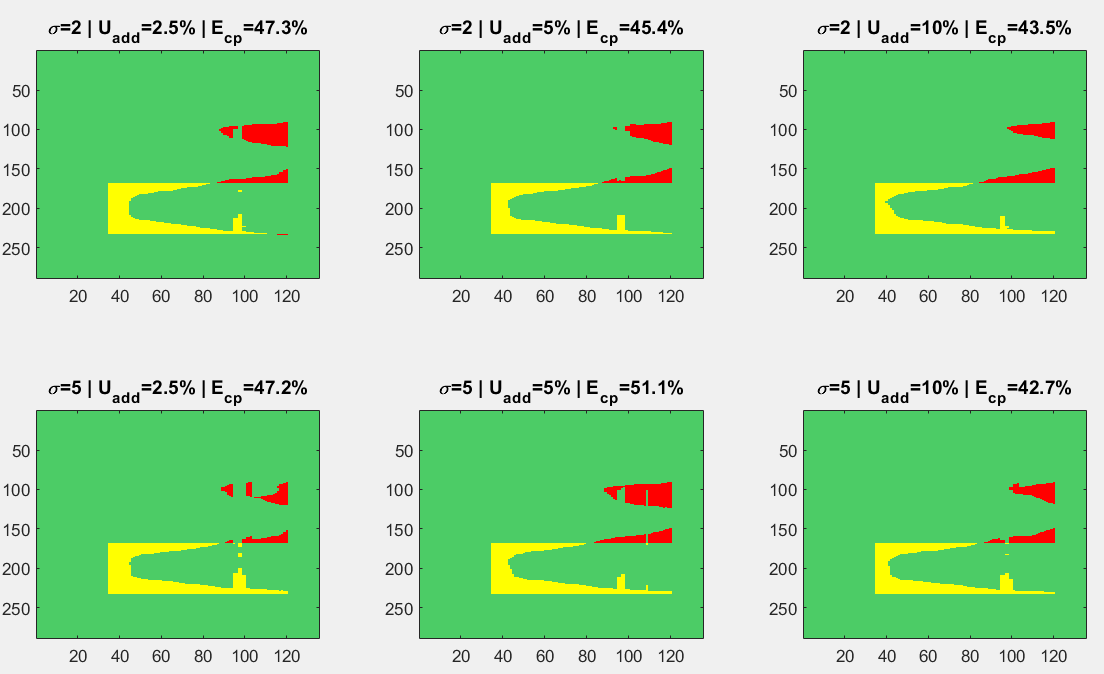
\includegraphics[width=6.8in]{figures/results_figures/Umul/cp_Umul_100_lambda_11.png}
\end{figure}
\begin{figure}[!h]
	\centering
	\caption{$\mathbf{U^{mul}=100\%}$. [0-10] knobs history plots : evolution with $U{add}$ and $\sigma$.}
	\label{fig:umulknobs100}
	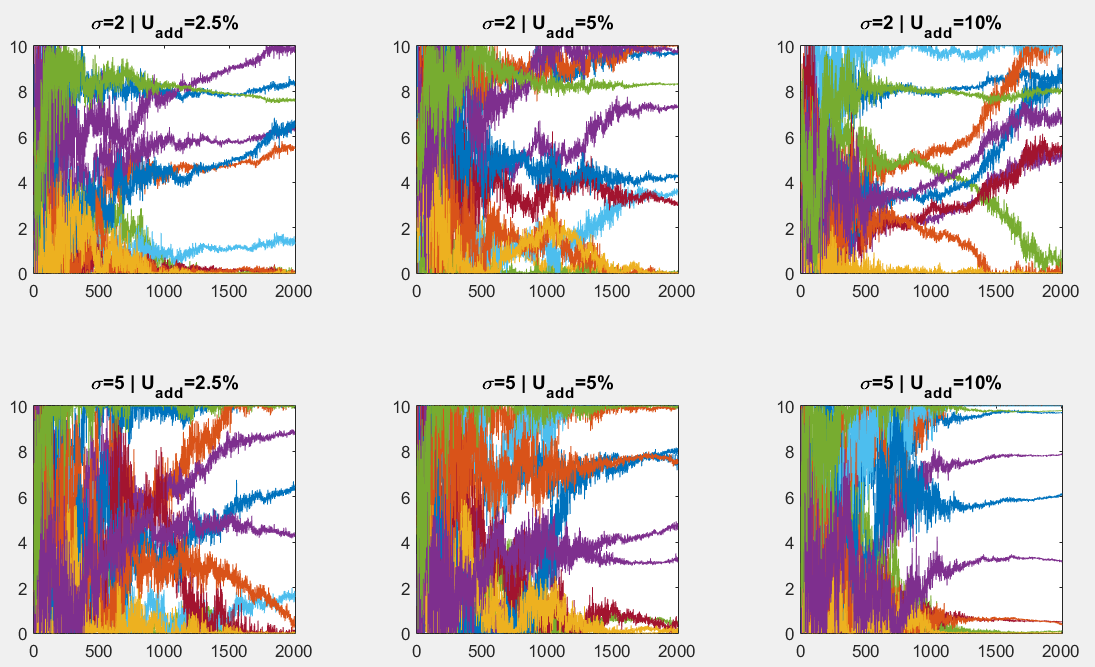
\includegraphics[width=7in]{figures/results_figures/Umul/knobs_Umul_100_lambda_11.png}
\end{figure}	

\emph{$U^{mul}=100\% $}: Fig. \ref{fig:umulcp100} shows too loose constraints lead too unlikely congestion situations. In this case, all the knob boundaries are their physical boundaries from $\mathscr{B}$ or are close to them. CMA-ES is not "guided" by boundaries that reflect likely traffic, it therefore finds a way of decreasing the congestion error by making non-physic "wholes" in the congestion patterns.\\
As we began to observe in Fig. \ref{fig:umulcp75}, the worst cases happen when $U^{add}$ is small. In this cases (first and second column), $6$ of the knobs boundaries are very loose, and $6$ are very tight : these are associated with small knob group flow demands, which always cause very tight boundaries with the multiplicative uncertainty.\\
Increasing $U^{add}$ diminishes this bad effect although it does not disappear : $U^{mul}=100\% $ is not a good choice.\\
This effect is not caused by the congestion threshold $d_{i}^{*}$ choice : full density or speed contour plots show the same non-physical undesirable congestion shapes. We see them in Fig. \ref{fig:badcontourplot}, a speed contour plot that intuitively reflects the congestion (located where the speeds are clearly slower).
We see in this figure that the traffic does not go smoothly from congested to non-congested, implying that the framed strange shape is not due to $d_{i}^{*}$ but to truly non-physic phenomena output by BeATS.\\

The knobs in Fig. \ref{fig:umulknobs100} do not behave as expected : most of them converge to their boundaries in all the cases, when we expected them to do the opposite, as we loosened the constraints. This illustrates that CMA-ES took advantage of the new non-realistic domains of the feasible space (i.e. far from the exact equation \ref{eq:balance}), close to its boundaries (many knobs converged to 0 !). There is therefore no advantage on setting $U^{mul}$ too large in terms of likelyhood of the resulting knob values.
\begin{figure}[!h]
	\caption{Speed contour plot. Example of non-physical effects on the congestion that appear when $U^{mul}$ is too large (100 \%)}
	\label{fig:badcontourplot}
	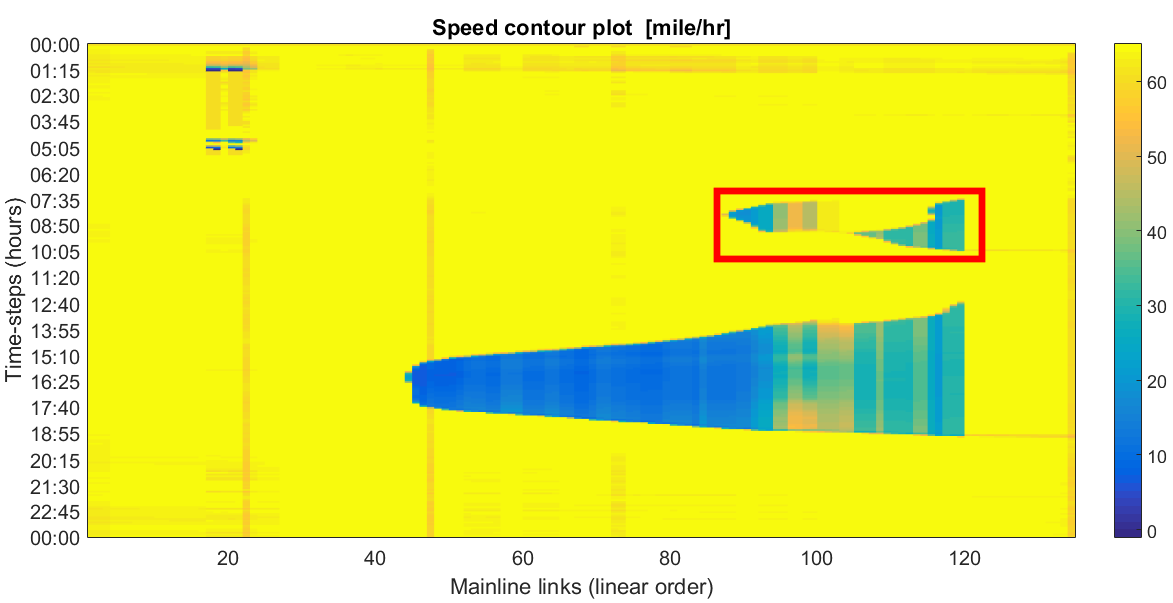
\includegraphics[width=7in]{figures/results_figures/Umul/badcontourplot.png}
\end{figure}
\\
\\
\emph{Conclusion}: Our experiments showed that there is a central domain for $U^{mul}$, at least as wide as $[50\% , 75\% ]$ in our case, that gives results of equivalent quality, the maximum allowed by the current templates shape. On the contrary, setting $U^{mul}$ to too small values, at least $U^{mul}\leq 25\% $ in our case, prevents the algorithm to grow the congestion satisfactorily. Finally, giving too much space to the knobs, at most $U^{mul}\geq 100\%$ in our case, leads to unfeasible congestion shapes and non-realistic extremal knobs, the algorithm taking advantage of the model/simulator imperfections. 